\section{Resultados}

Se implementararon los algoritmos de gradiente conjugado con los calculos de $\beta$ para FR, PR, HS y FR-PR. En todos los casos se partio desde un punto inicial aleatorio dado por la ecuación .

\begin{equation*}
    X_0 = \{x_{i,j} \in \mathit{U}(0,1) \text{ para } 1<i<n\;\; 1<j<m\}
\end{equation*}

Se usaron los valores de $0.1, 0.5, 1$ y $5$ para la ecuación \ref{eq:cost_function}.

\subsection{Evolución temporal de la solución}

Realizando comparaciones de los valores de la función y la norma del gradiente en cada iteración se obtuvieron las figuras \ref{fig:function_gradient}.

\begin{figure}[H]
    \centering
    \begin{subfigure}{8.4cm}
        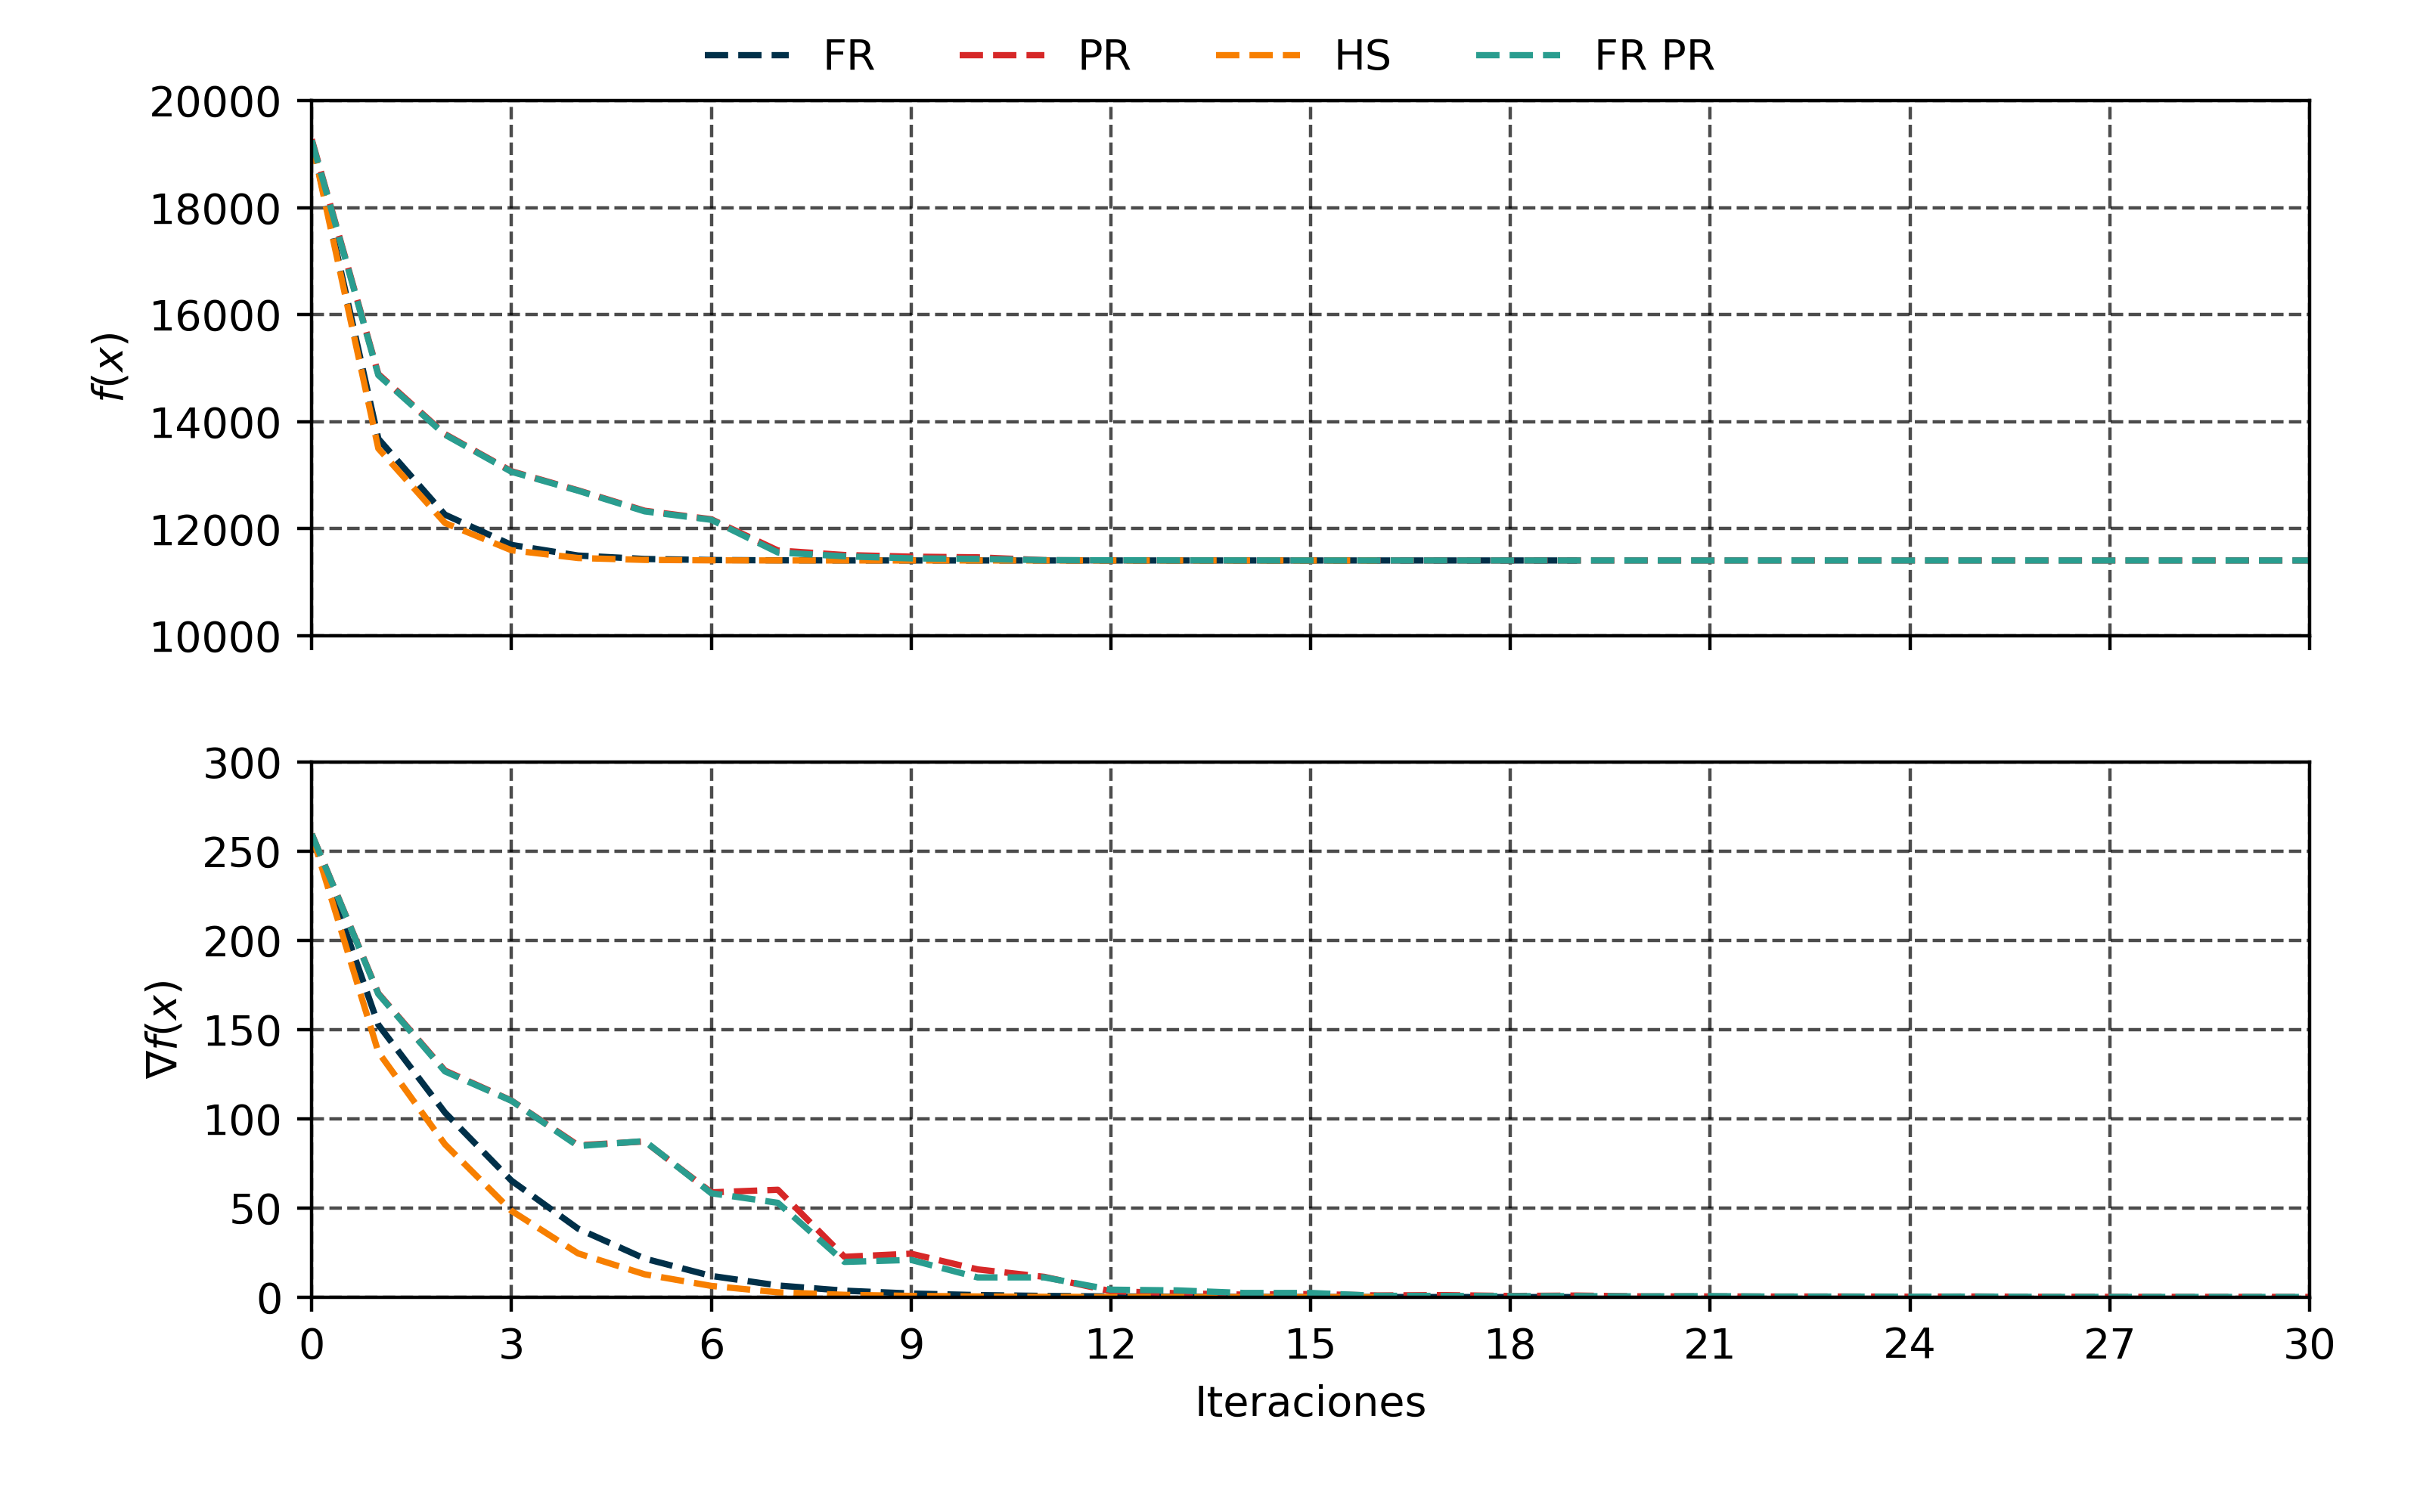
\includegraphics[width=1\textwidth]{Graphics/lambda_1.png}
        \caption{$\lambda = 0.1$}
    \end{subfigure}
    \begin{subfigure}{8.4cm}
        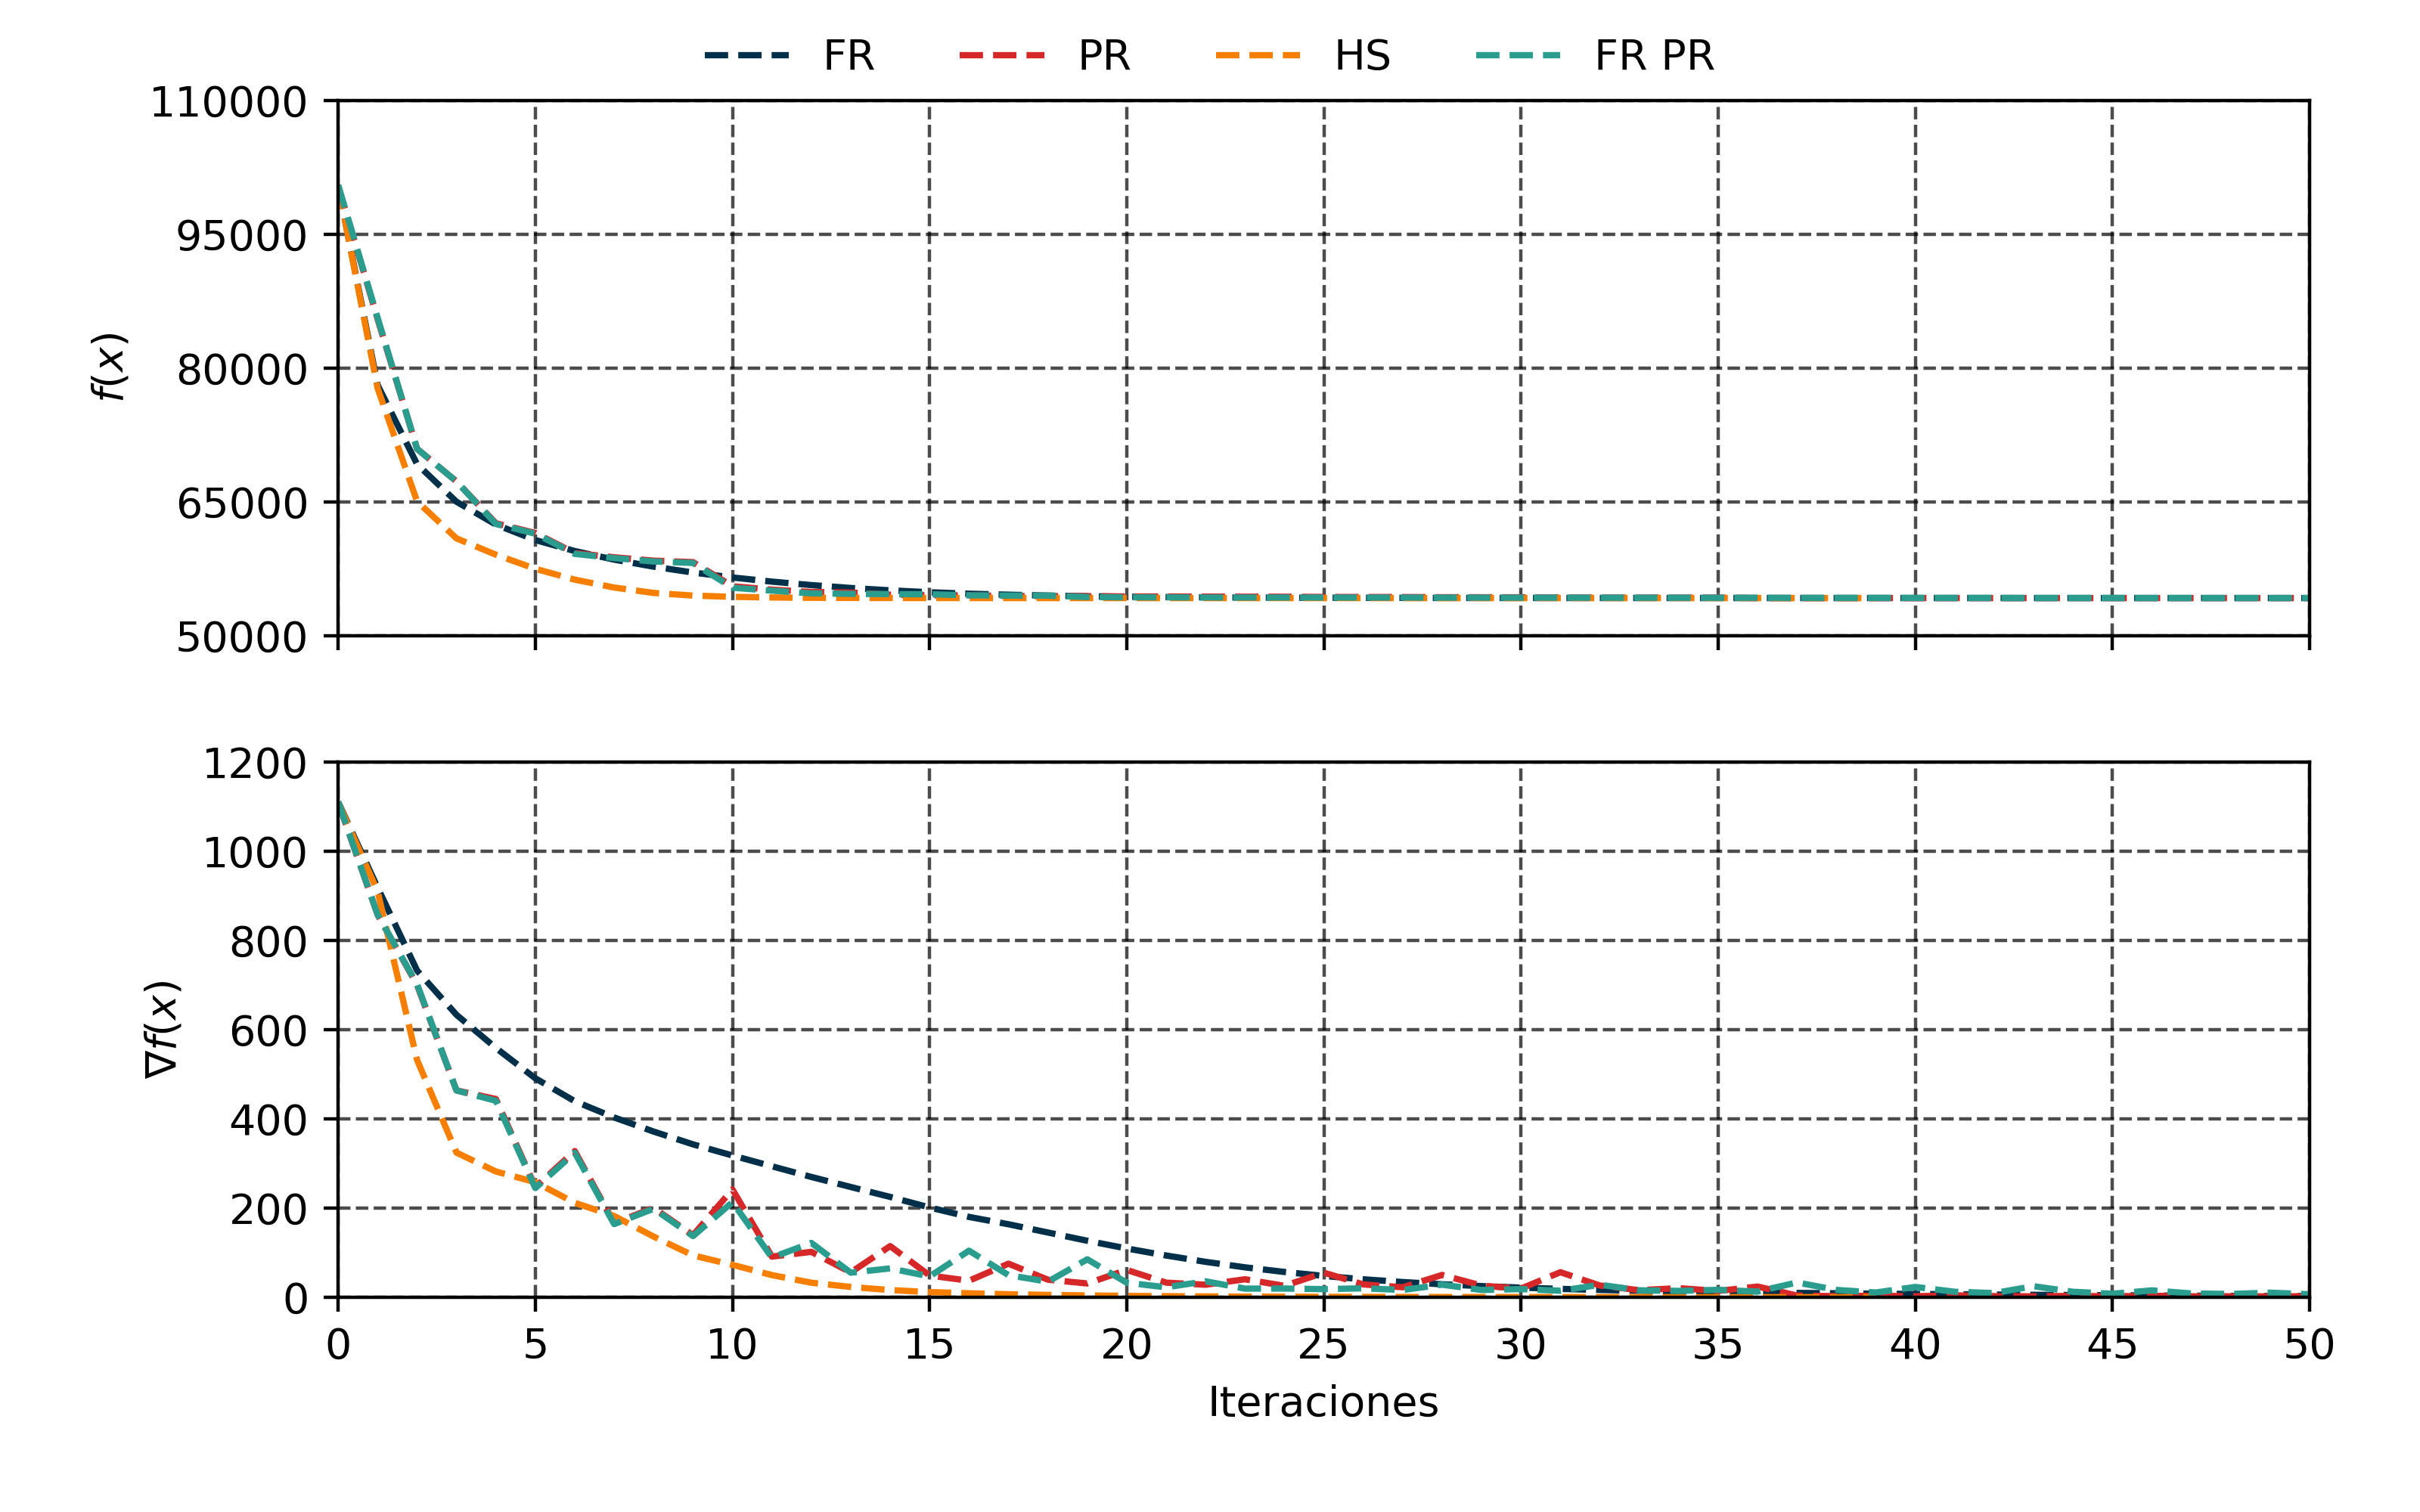
\includegraphics[width=1\textwidth]{Graphics/lambda_2.png}
        \caption{$\lambda = 0.5$}
    \end{subfigure}
    \begin{subfigure}{8.4cm}
        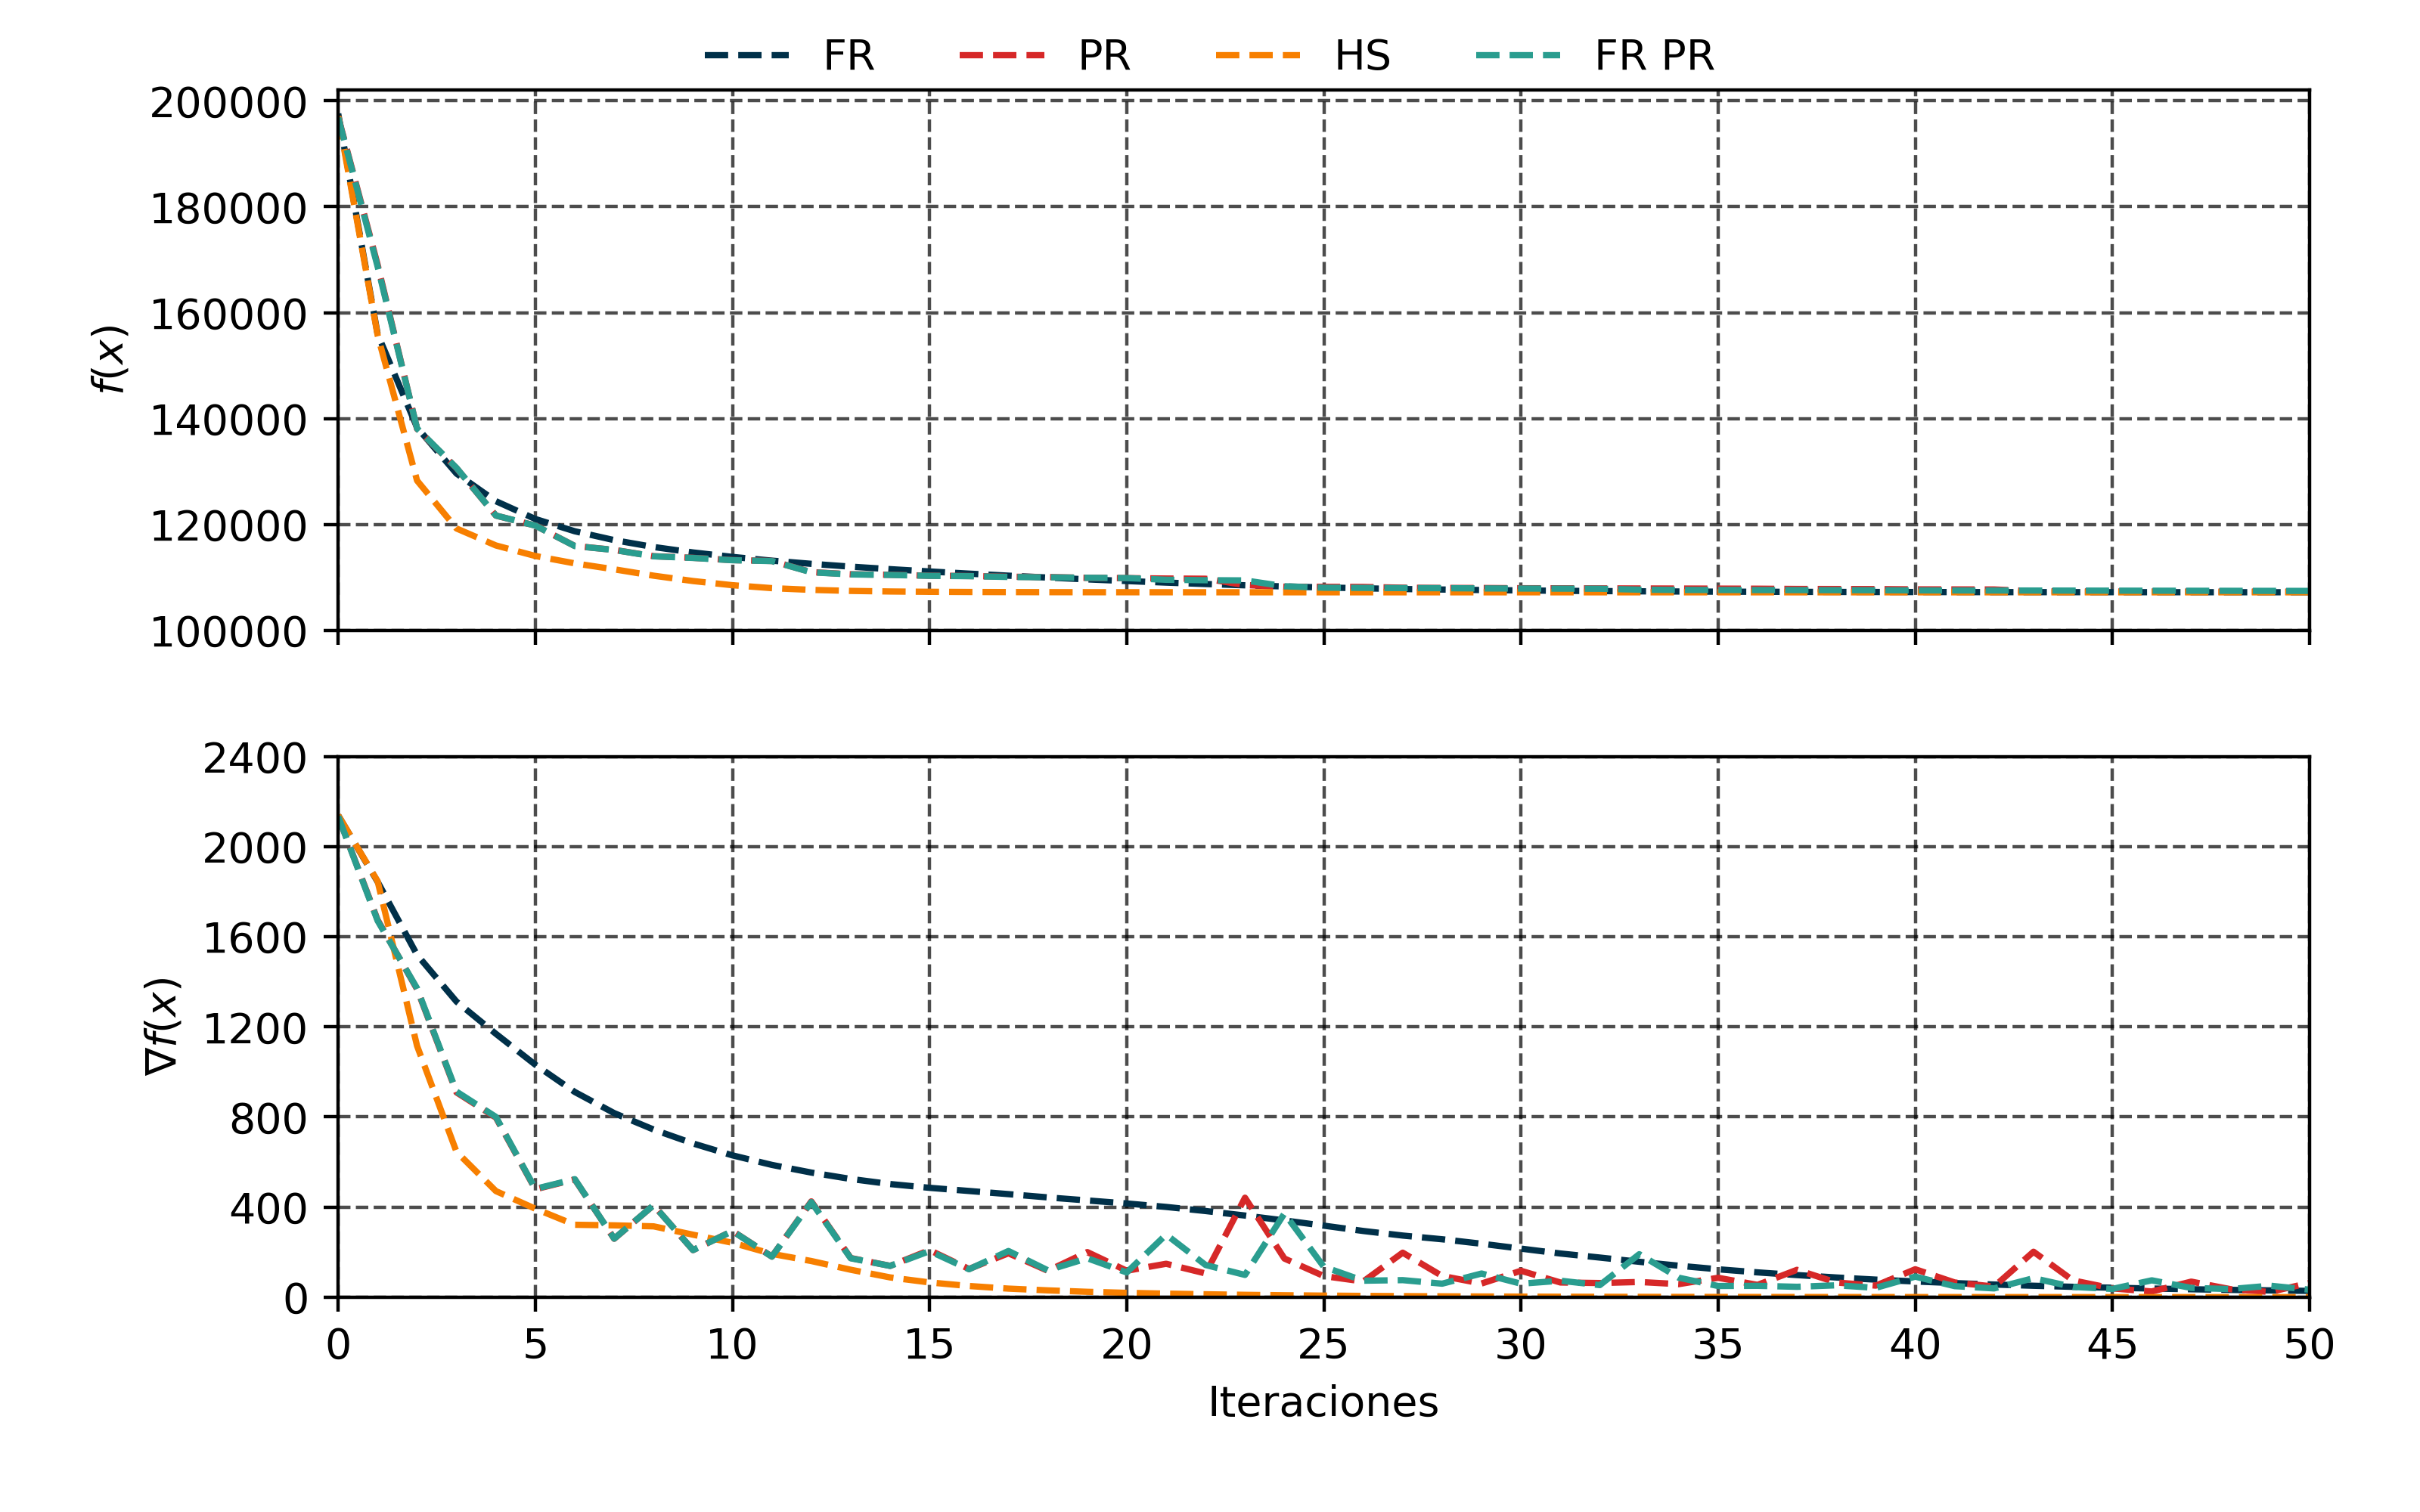
\includegraphics[width=1\textwidth]{Graphics/lambda_3.png}
        \caption{$\lambda = 1$}
    \end{subfigure}
    \begin{subfigure}{8.4cm}
        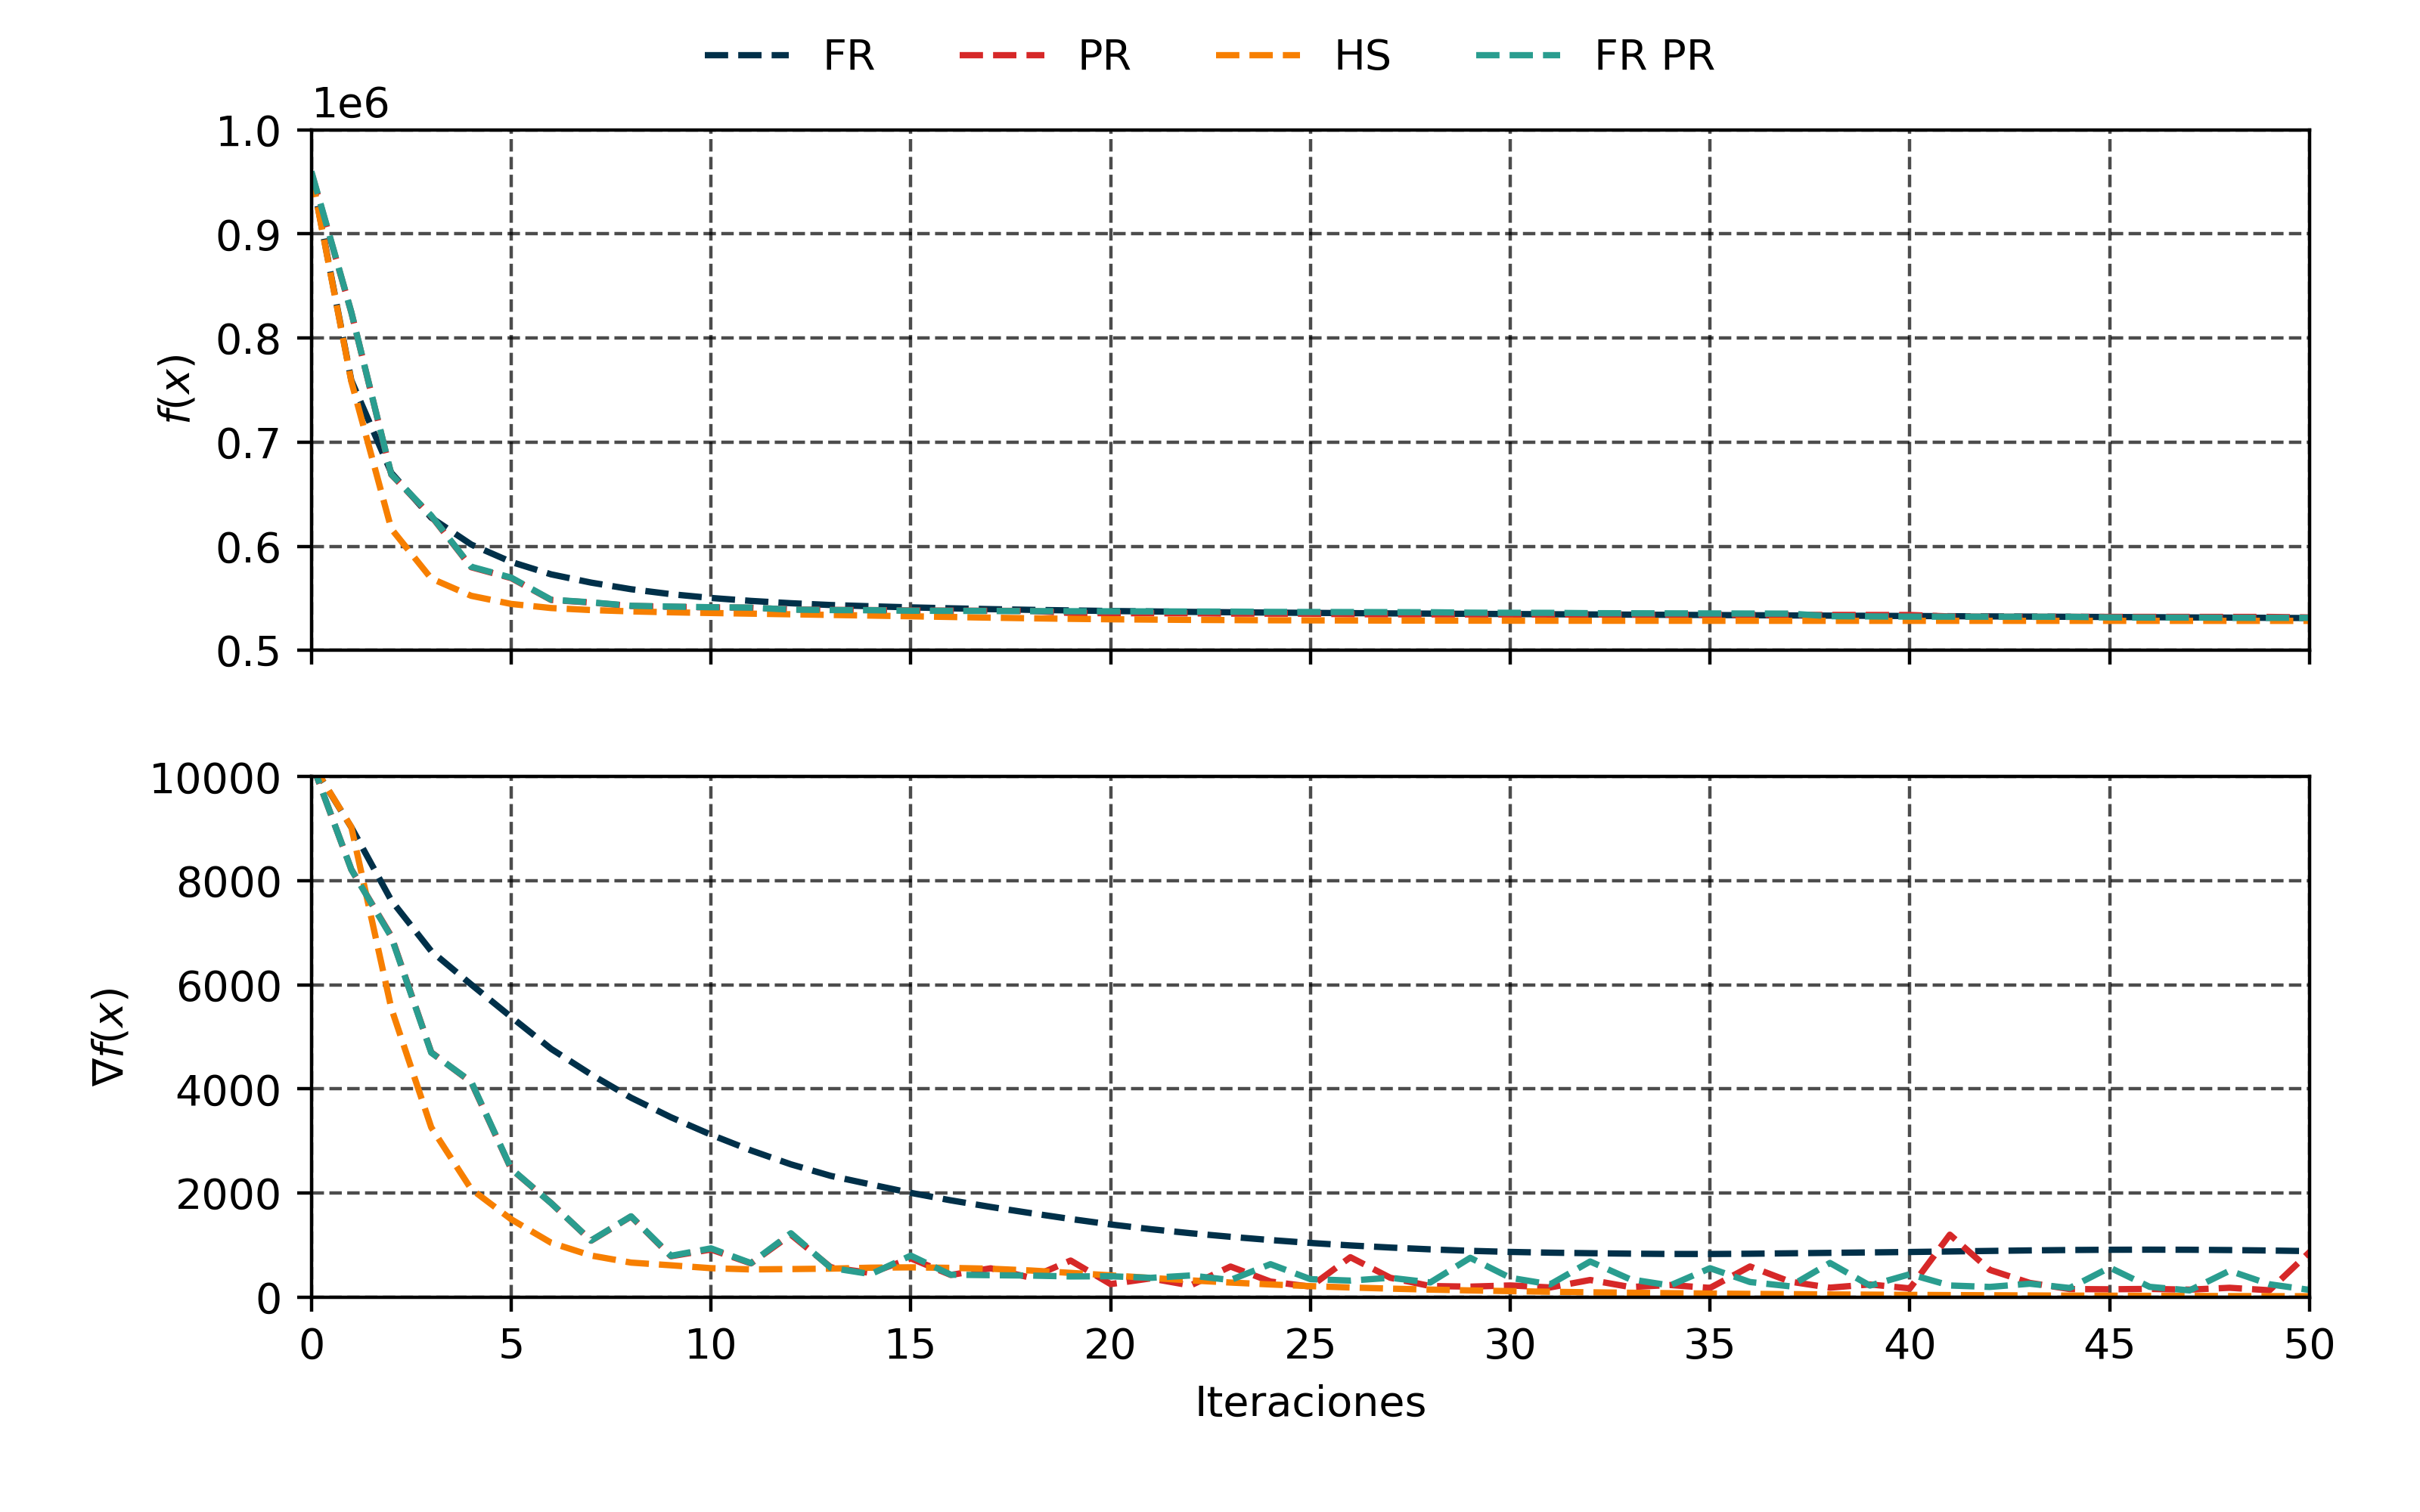
\includegraphics[width=1\textwidth]{Graphics/lambda_4.png}
        \caption{$\lambda = 5$}
    \end{subfigure}
    \caption{Valor de la función y norma del gradiente en cada iteración para el método de gradiente conjugado con pasos FR, PR, HS y FR-PR para $lambda=\{0.1, 0.5, 1,2\}$}
    \label{fig:function_gradient}
\end{figure}

\subsection{Suavizado de imágenes}

En la figura \ref{fig:images} se visualizan los resultados al introducir una imagen en el parámetro $g$ de la ecuación \ref{eq:cost_function} para los métodos FR, PR, HS y FR-PR.

\begin{figure}[H]
    \centering
    \begin{subfigure}{16cm}
        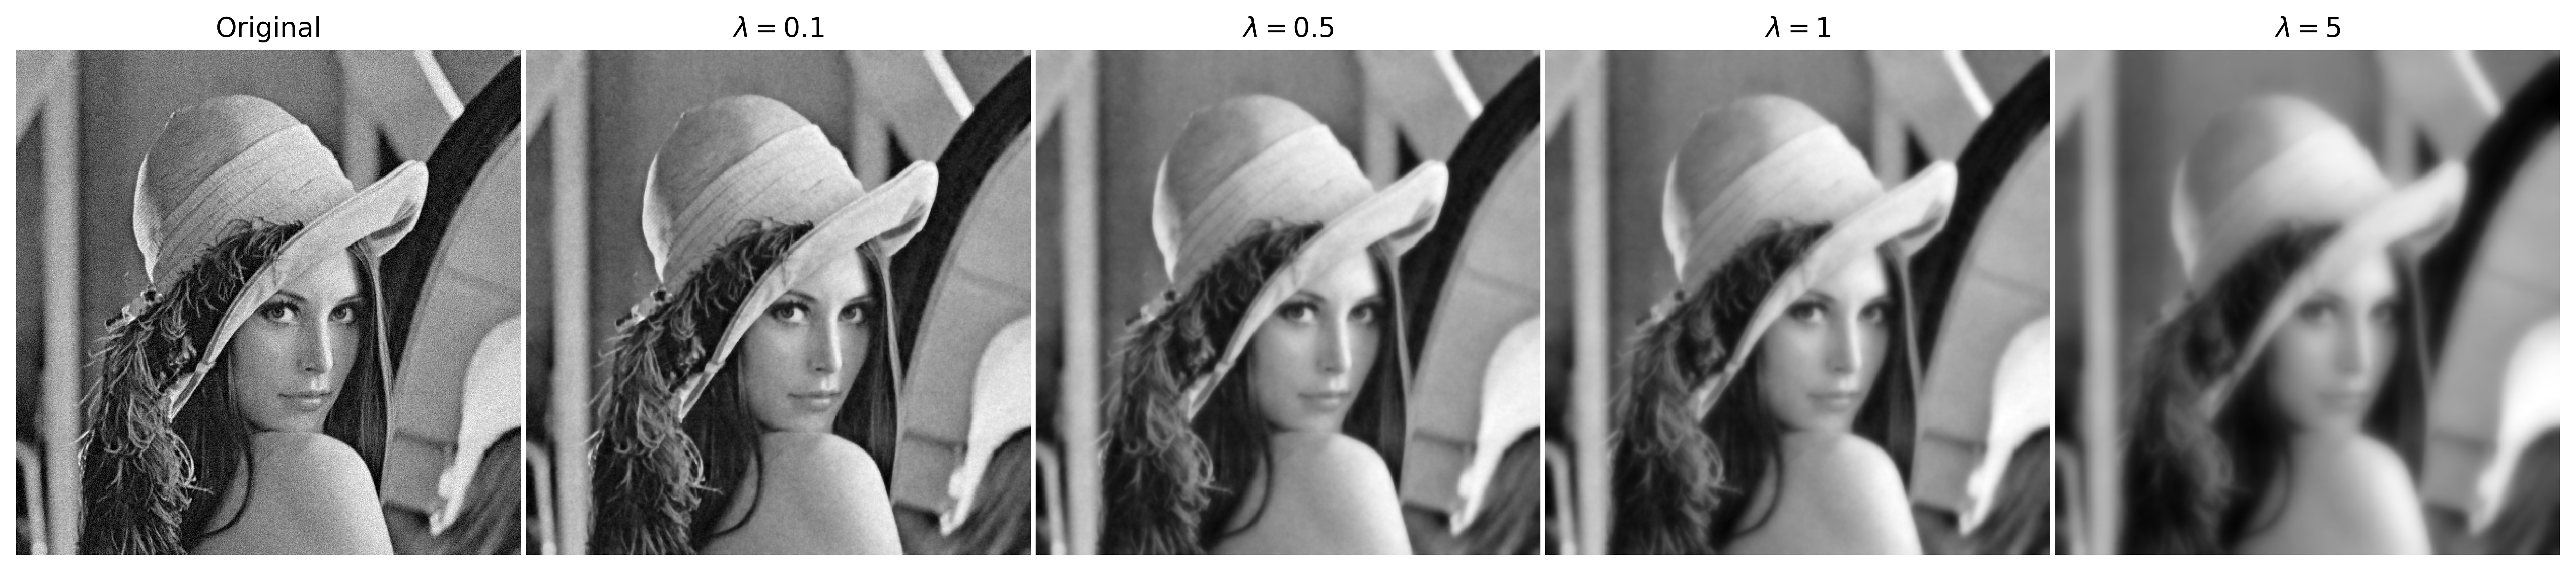
\includegraphics[width=1\textwidth]{Graphics/FR.png}
        \caption{Método FR}
    \end{subfigure}
    \begin{subfigure}{16cm}
        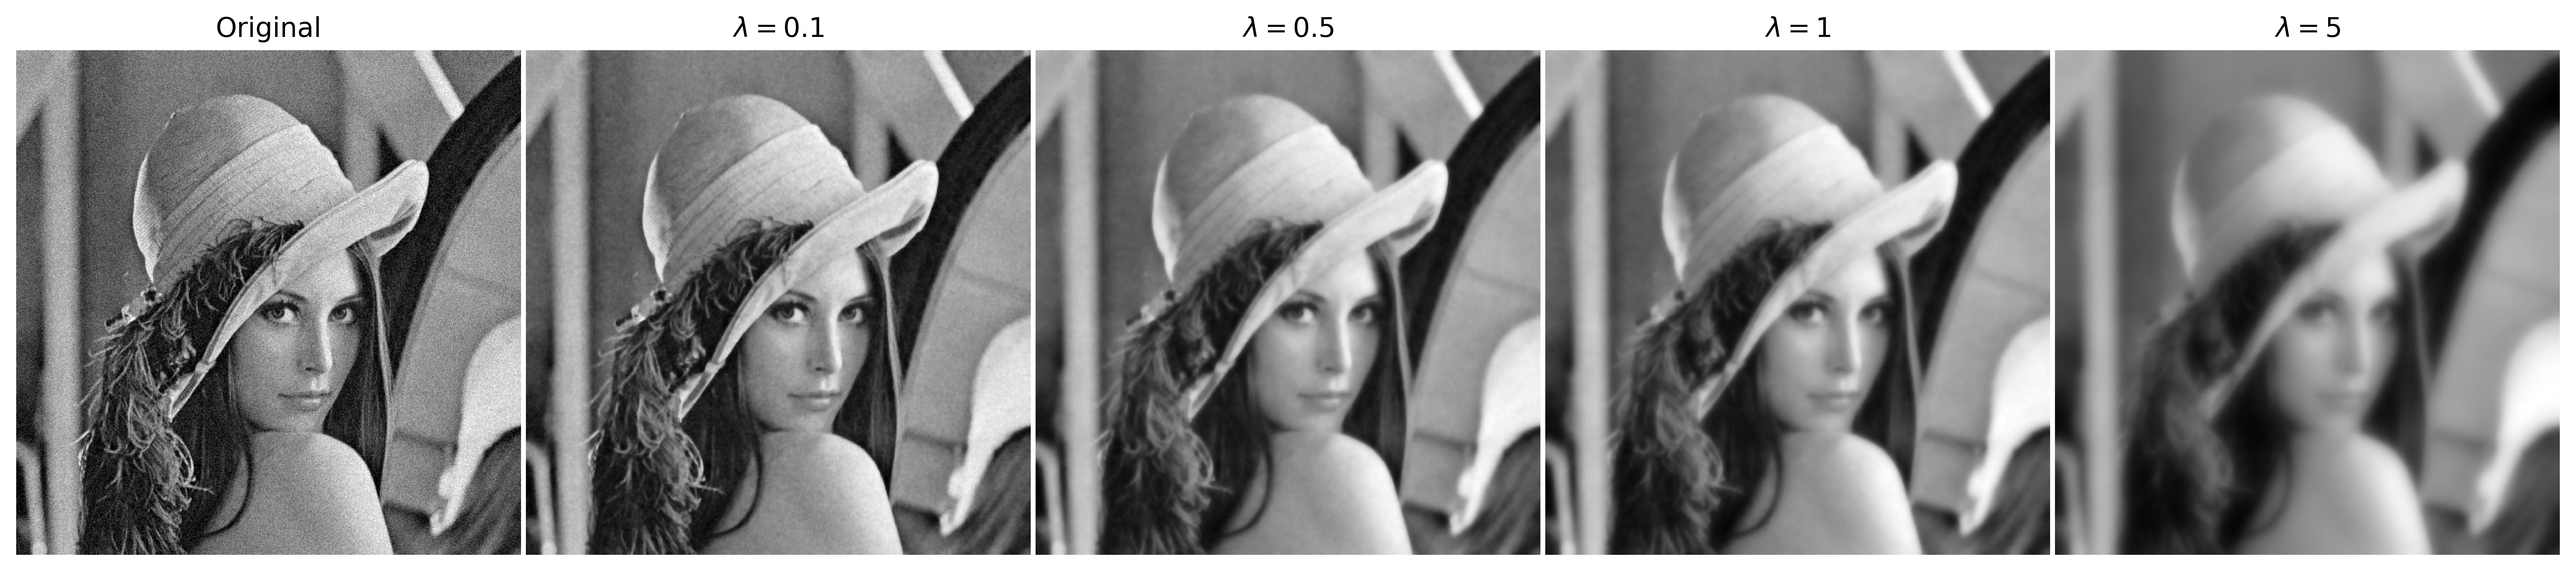
\includegraphics[width=1\textwidth]{Graphics/PR.png}
        \caption{Método PR}
    \end{subfigure}
    \begin{subfigure}{16cm}
        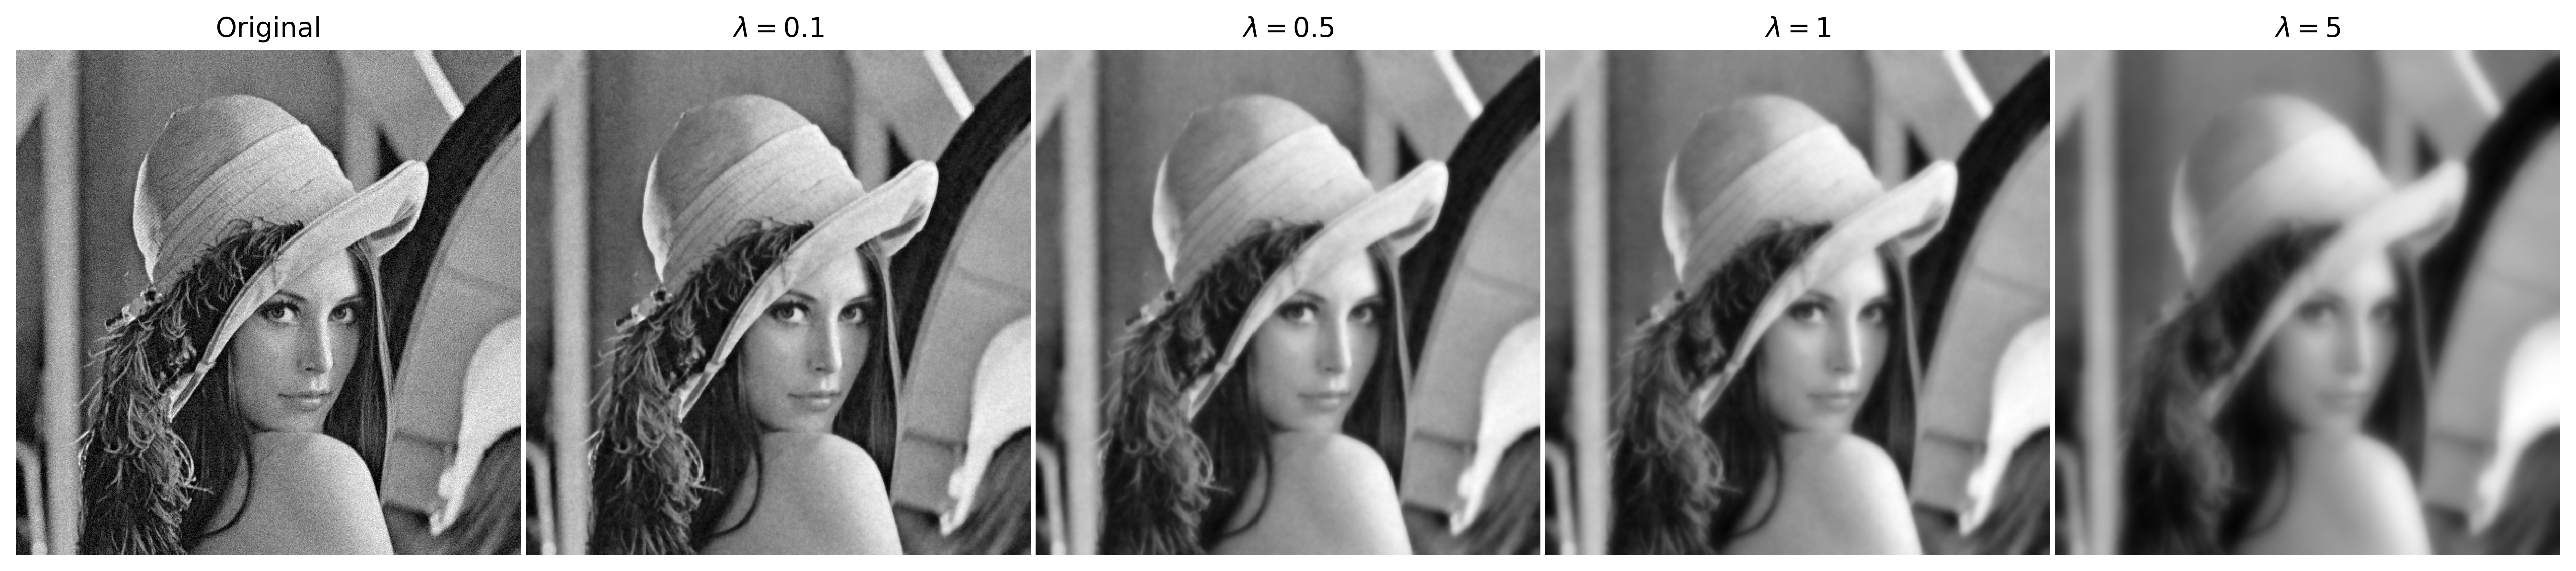
\includegraphics[width=1\textwidth]{Graphics/HS.png}
        \caption{Método HS}
    \end{subfigure}
    \begin{subfigure}{16cm}
        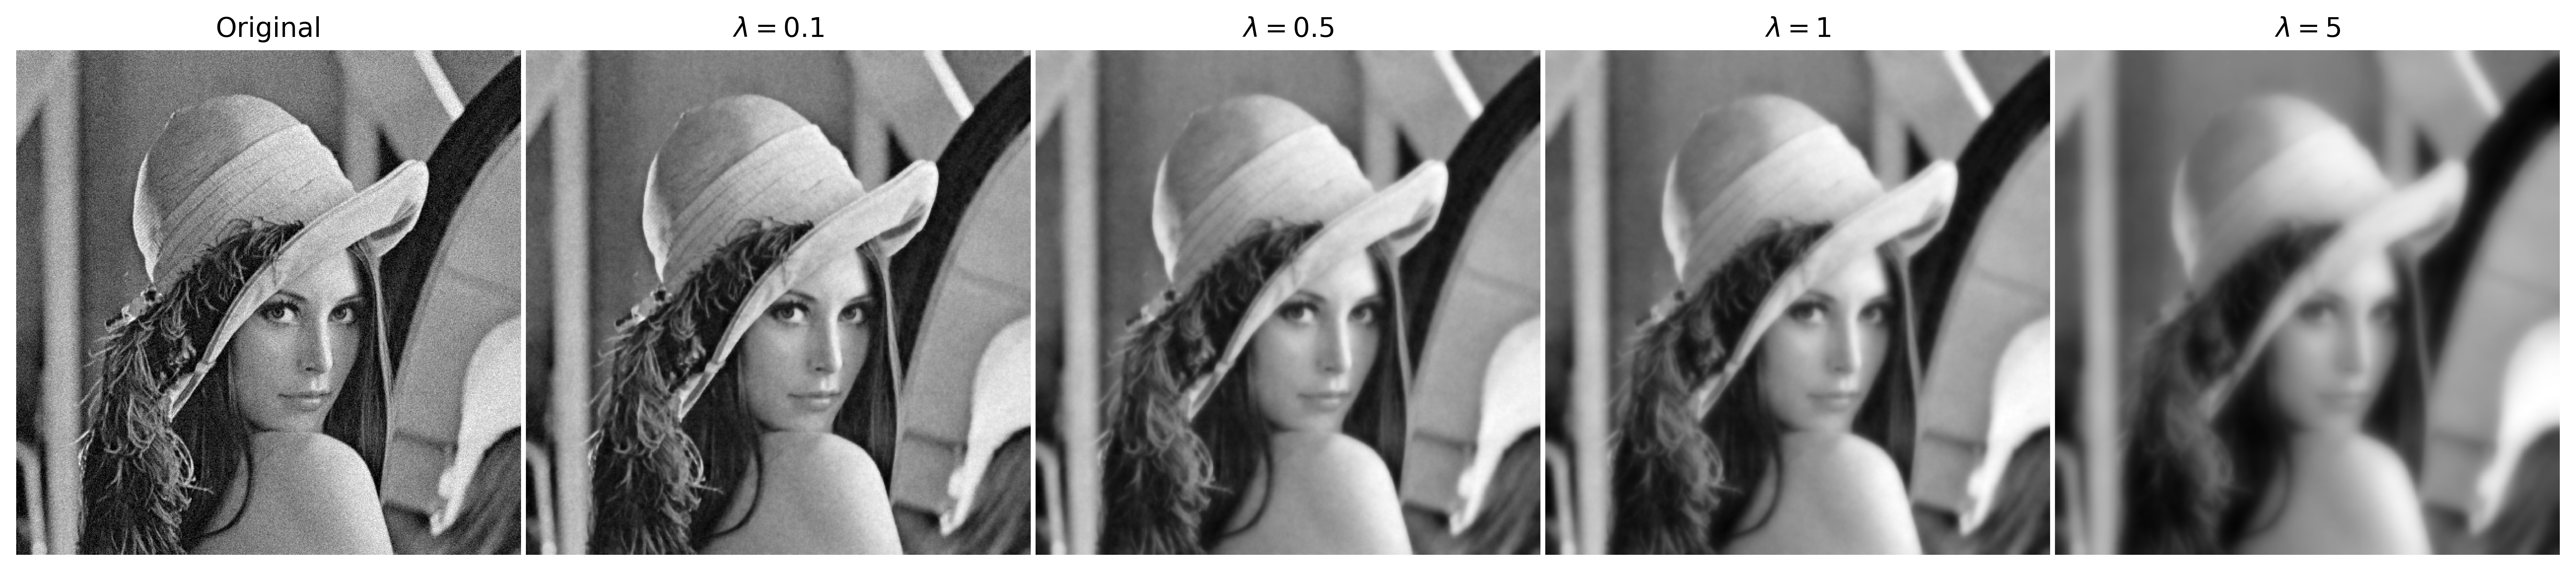
\includegraphics[width=1\textwidth]{Graphics/FR PR.png}
        \caption{Método FR-PR}
    \end{subfigure}
    \caption{Resultados de las imagenes para cada método y $lambda$.}
    \label{fig:images}
\end{figure}